\section*{Excersises 1}
\begin{itemize}
\item
Exercise 1-1:\\
Verify that the vector addition is associative,i.e., 
\[
	\fat{a}+(\fat{b}+\fat{c})=
		(\fat{a}+\fat{b})+\fat{c}
\]
using graphic representation of vectors. 
\item
Exercise 1-2:\\
For vectors $\fat{a}$ and $\fat{b}$ given in Fig.\ref{fig:fig1_1}, 
work out $\fat{a}+\fat{b}$ by the component based 
		method when  $|\fat{a}|=1$ and $|\fat{b}|=2$.
		Also, obtain $|\fat{a}+\fat{b}|$ numerically.
\item
Exercise 1-3:\\
		For vectors given in Fig.\ref{fig:fig1_2} Prove that 
	\[
		\fat{a}+\fat{b}+\fat{c}=\fat{0}
	\]
		if $|\fat{a}|=|\fat{b}|=|\fat{c}|$.
\item
Exercise 1-4:\\
Suppose that a perfectly rigid bar AB is supported horizontally by a wall
 as shown in Fig.\ref{fig:fig1_3}, and is subjected to infinitely many 
vertical forces $\fat{f}_i (i=1,2,...)$ whose magnitude decreases monotonically as 
\[
 \frac{
	|\fat{f}_{i+1}|
	}{
	|\fat{f}_i|
}
	=\frac{9}{10} 
\]
Determine the direction and the magnitude of the total force acting on the bar. 
\item
Exercise 1-5:\\
	Suppose that an iron weight is hung from a ceiling by a string AB as shown in Fig.\ref{fig:fig1_4}-(a). 
	Determine the magnitude of the horizontal force $F$ required to hold the weight as 
	in the position shown in Fig\ref{fig:fig1_4}-(b).
	Note that $m$ is mass and $g$ is gravity constant.  
\end{itemize}
\begin{figure}[h]
	\begin{center}
	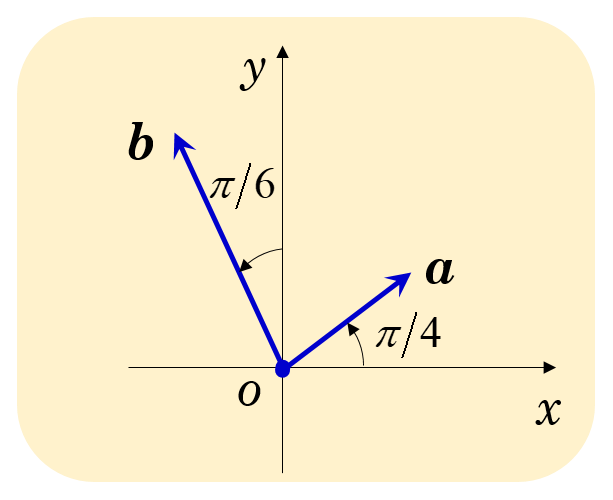
\includegraphics[width=0.4\linewidth]{fig1_1.eps} 
	\end{center}
	\caption{Vectors $\fat{a}$ and $\fat{b}$ in 2-dimensional space with an
	xy Cartesian coordinate system.}
	\label{fig:fig1_1}
\end{figure}
\begin{figure}[h]
	\begin{center}
	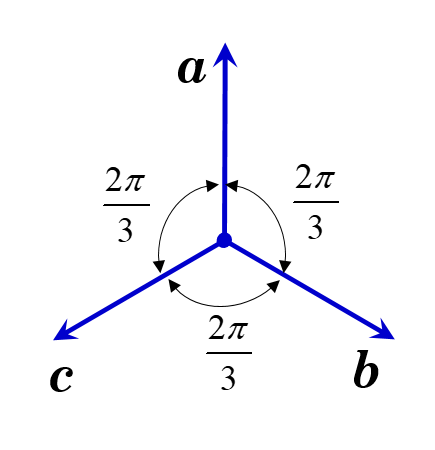
\includegraphics[width=0.4\linewidth]{fig1_2.eps} 
	\end{center}
	\caption{Vectors $\fat{a}, \fat{b}$ and $\fat{c}$ of equal magnitude.} 
	\label{fig:fig1_2}
\end{figure}
\begin{figure}[h]
	\begin{center}
	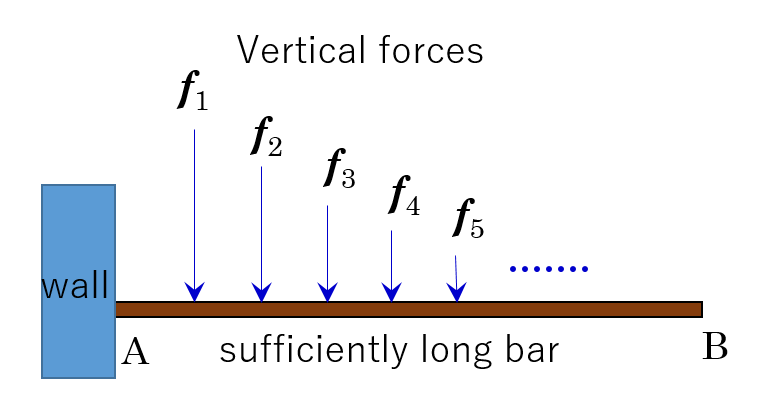
\includegraphics[width=0.6\linewidth]{fig1_3.eps} 
	\end{center}
	\caption{Infinitely many downward forces acting to a horizontally supported bar AB.}
	\label{fig:fig1_3}
\end{figure}
\begin{figure}[h]
	\begin{center}
	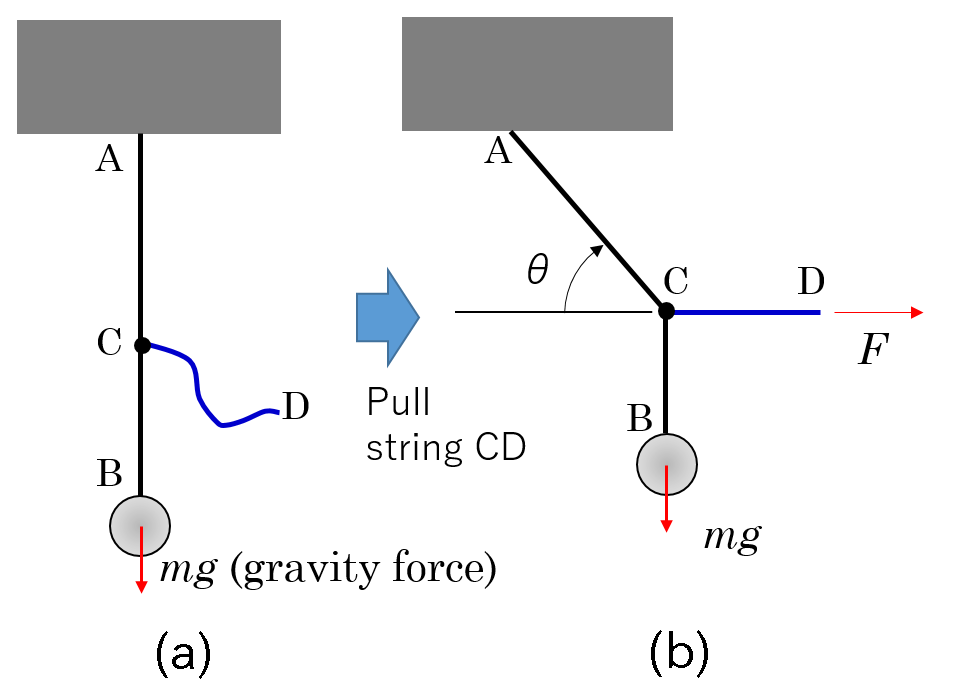
\includegraphics[width=0.6\linewidth]{fig1_4.eps} 
	\end{center}
	\caption{An weight of mass $m$ hung from a ceiling by a string AB.} 
	\label{fig:fig1_4}
\end{figure}
%%%%%%%%%%%%%%%%%%%%%%%%%%%%%%%%%%%%%%%%%%%%%%%%%%%%%%%%%%%%%%%%
